\documentclass[ngerman]{article}

\usepackage[utf8]{inputenc}
\usepackage[ngerman]{babel}

\usepackage{listings}
\usepackage{color}
\usepackage{graphicx}

\author{Hong-Khoan Quach, Marek Kubica, Julius Adorf \\ Technische Universität München}

\title{ETI-Großprojekt 8\\
       Sommersemester 2009 \\
       {\bf Das Carrierpigeon-Projekt}
}

\date{\today}

% cheat a little bit
% code samples should not be split
\setlength{\headheight}{-20pt}
\setlength{\textheight}{590pt}

% colorize code samples
\lstset{language=C}
\lstset{
    basicstyle=\small,
    keywordstyle=\color[rgb]{0.1,0.1,0.8}
    }

\setlength{\parindent}{0cm}
\setlength{\parskip}{1em}

\begin{document}

\maketitle

\begin{abstract}
Das Carrierpigeon-Projekt ist ein studentisches Lernprojekt, dessen Ziel es war,
ein System zu erstellen, in dem man mit einem Handy mittels Bluetooth
Nachrichten an einen elektronischen Briefkasten zu senden. Auf dem
elektronischen Briefkasten kann man die empfangenen Nachrichten anzeigen
und anschließend auch löschen. Der Briefkasten besteht aus einem Mikrocontroller,
einer kleinen Flüssig\-kristall\-an\-zeige, einigen Tasten und einem
Bluetooth-Modul.
\end{abstract}


\section{Motivation}

Das Carrierpigeon-Projekt ist 2009 am Lehrstuhl für Rechnertechnik und Rechnerorganisation der Technischen
Universität München im Rahmen eines studentischen Praktikums entstanden. Uns ging es darum,
zu untersuchen, wie man mit einem Mikrocontroller über Bluetooth mit Geräten in der Umgebung
kommunizieren kann, und zudem eine Anwendung zu entwickeln, die diese Form der Kommunikation
integriert. Es ging nicht darum, einen Prototypen für ein markttaugliches System zu erstellen.
Stattdessen der Lerneffekt und die Lösung der technischen Fragestellungen im Vordergrund.

Trotzdem haben wir in der Entwicklung nicht nur experimentiert, sondern uns an einer bestimmten
Idee orientiert, um klare Anforderungen an das System zu erhalten. Begonnen hat das Projekt mit
folgenden Anwendungsfall:
\begin{quote}

Alpha möchte Beta besuchen. Beta ist leider nicht da. Daher möchte Alpha eine Nachricht
mit seinem Handy auf Betas elektronischen Briefkasten hinterlassen. Kommt Beta nun zurück,
so kann Beta sich die empfangenen Nachrichten durchlesen.
\end{quote}

\section{Begriffe}

In dem gerade beleuchteten Szenario treten verschiedene Rollen und technische Komponenten auf.
Die beiden technischen Komponenten sind der \textit{Briefkasten} und das \textit{Mobiltelefon}.
Den \textit{Sender} ist der Benutzer, der vom Mobiltelefon aus Nachrichten sendet. Den Benutzer,
an den die Nachrichten adressiert sind und diese lesen kann, nennen wir \textit{Empfänger}.

Die Rollen des Senders stellen einige Anforderungen an das Programm auf dem Mobiltelefon.
Als Sender soll man auf einfache Art und Weise eine Nachricht eingeben können. Als Sender soll
man einen Briefkasten aus einer Liste wählen und diesem eine Nachricht senden können.

Analog dazu legt die Rolle des Empfängers die Anforderungen an den Briefkasten fest:
Als Empfänger bekommt man die neueste Nachricht an\-gezeigt.
Man soll eine beliebige der gespeicherten Nachrichten anzeigen können. Schließlich soll man als
Empfänger gespeicherte Nachrichten löschen können.


\section{Architektur}

        \subsection{Hardware-Architektur des Briefkastens}

Der Briefkasten besteht aus einem ATmega8515-Mikrocontroller, der über Ports eine
ST565-Flüssigkristallanzeige bedienen kann. Der Mikrocontroller ist mit einen
UART-Baustein - also über eine serielle Schnittstelle - mit dem BTM-222-Bluetooth-Modul
kommunizieren. Im Folgenden gibt ein Schaubild eine grobe Übersicht der wichtigsten 
Hardware-Elemente. Für eine genaue Spezifikation sei hier auf die Refernenzhandbücher des ATmega8515, 
des ST565 bzw. des BTM-222 verwiesen. 

\begin{figure}[h!] \begin{center}
    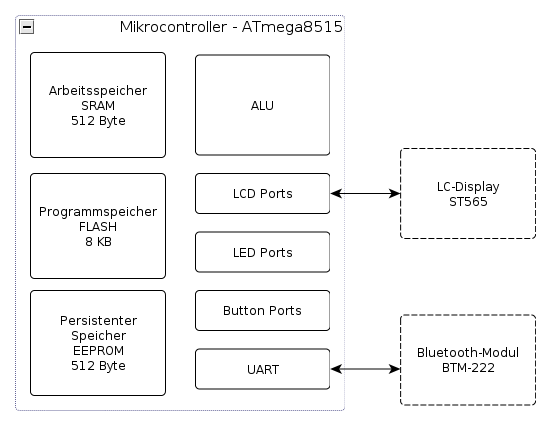
\includegraphics[width=0.6\textwidth]{media/letterbox-atmega-arch}
\end{center} \end{figure}

Die einzelnen Bauteile kommunizieren über einen 8-bit-Datenbus. Besonders auffällig ist,
dass der ATmega8515 eine Harvard-Architektur darstellt. Im Gegensatz zu einem
Von-Neumann-Rechner liegen in einer Harvard-Architektur Daten und Programm in
unterschiedlichen Speichern. Die Programme liegen im vergleichsweise großzügig bemessenen
Programmspeicher (FLASH), die Programmdaten, der Stack und der Heap teilen sich den
mit 512 Byte knapp bemessenen Datenspeicher (SRAM). Für die persistente Speicherung
von Daten über Zeiten ohne Stromzufuhr hinweg existiert ein dritter persistenter Speicher (EEPROM).
Ohne Erweiterung kann man auch im EEPROM nur 512 Byte speichern.


        \subsection{Software-Architektur des Briefkastens}

Auf der Hardware des Briefkastens läuft ein C-Programm, das aus verschiedenen, handlichen Modulen
zusammen gesetzt ist. Eine Schaubild illustriert den Zweck, die verschiedenen Abstraktionsebenen
und das Zusammenspiel der einzelnen Module.

\begin{figure}[h!] \begin{center}
    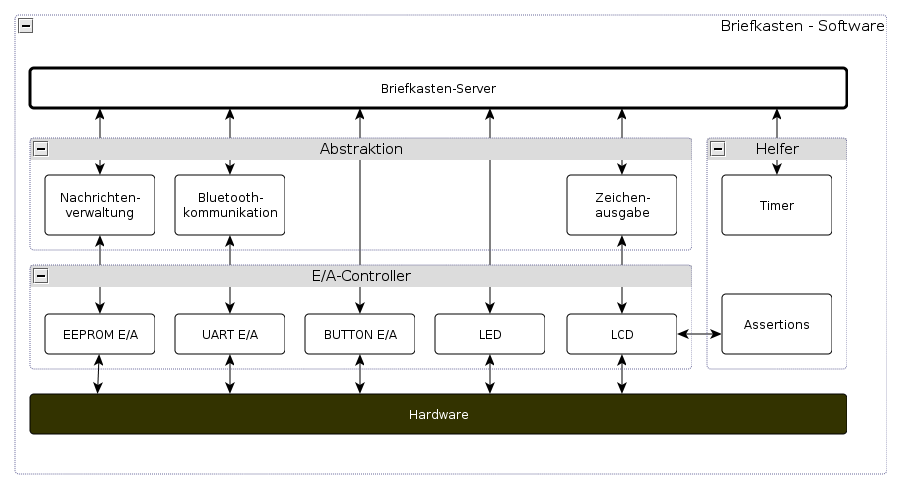
\includegraphics[width=\textwidth]{media/letterbox-arch}
\end{center} \end{figure}

Direkt über der Hardware liegen die E/A-Controller. Das sind Module, die alle Formen von Eingabe
und Ausgabe steuern und von der tatsächlichen Hardware abstrahieren. Über den E/A-Controllern
existieren Module, die für Abstraktion sorgen, die über die einfachen Aufgaben der E/A-Controller
hinausgeht. Für manche Module, wie z.B. die Controller der Tasten oder Leuchtdioden ist eine weitere
Abstraktion nicht notwendig. Ganz oben liegt das Serverprogramm des Briefkastens, das sich auch
eines Timers bedient. Für Zwecke des Debuggings besteht ein Assertion-Modul, das mangels besserer
Ausgabemöglichkeiten vom LCD abhängig ist.


        \subsection{Software-Architektur des Mobiltelefons}

Die Applikation für das Mobiltelefon ist plattformunabhängig und auf Betriebssystemen und
Mobiltelefonen ganz verschiedener Hersteller laufen. Sie ist in Java implementiert und baut
auf drei Spezifikationen auf. Wie diese implementiert sind, interessiert uns nicht weiter.

\begin{figure}[h!] \begin{center}
    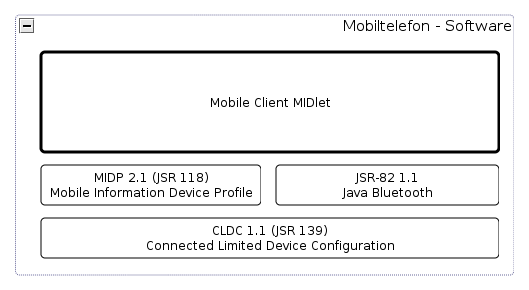
\includegraphics[width=0.7\textwidth]{media/mobile-client-arch}
\end{center} \end{figure}

Die Installation der Applikation erfolgt je nach Handy-Hersteller unterschiedlich. Auf den
meisten Geräten lässt sich die Applikation sehr einfach installieren, in dem man sie z.B.
über Bluetooth an das Handy schickt. 


\section{Briefkasten}

Die gesamte Software auf dem Briefkasten ist in C programmiert. Änderungen
am Code sollen sich möglichst nur lokal auswirken. Das Finden und Ausbessern von 
Schwachstellen wird dadurch erleichtert, dass das Programm in einzelne Module
mit unterschiedlichen Verantwortlichkeiten aufgeteilt ist.

\begin{tabular}{|l|l|l|}
    \hline
    {\bf Modul} & {\bf Pfad} & \\
    \hline
    \hline
    EEPROM E/A & {\tt letterbox/eeprom/eeprom.h} & \\
    \hline
    UART E/A & {\tt letterbox/uart/uart.h} & \\
    \hline
    BUTTON E/A & {\tt letterbox/buttons/buttons.h} & \\
    \hline
    LED & {\tt letterbox/buttons/led.h} & \\
    \hline
    LCD & {\tt letterbox/lcd/lcd.h} & \\
    \hline
    Zeichenausgabe & {\tt letterbox/lcd/text.h} & \\
    \hline
    Bluetooth-Kommunikation & {\tt letterbox/uart/bt.h} & \\
    \hline
    Nachrichtenverwaltung & {\tt letterbox/message/message.h} & \\
    \hline
    Assertions & {\tt letterbox/assert/assert.h} &  \\
    \hline
    Timer & {\tt letterbox/timer/timer.h} & \\
    \hline
    Server  & {\tt letterbox/main.c} & \\
    \hline
\end{tabular}

Zu dem C-Programm müssen wir ehrlicherweise anmerken, dass wir uns nicht besonders
um programmweite Konsistenz bei den verwendeten Datentypen gekümmert haben. Im Folgenden
kommen nun die Modulbeschreibungen. Sie enthalten je eine Übersicht der deklarierten
Prozeduren um einen Zusammenhang zur tatsächlichen Implementierung herzustellen.

\subsection{E/A-Controller}

Die E/A-Controller sind dafür zuständig, die Hardware auf der Ebene von Bits und Bytes zu
steuern. Zu ihren Aufgaben gehört das Auslesen der Tasten, das An-
und Ausknipsen der Leuchtdioden,  das Beschreiben des Speichers,
die Ansteuerung des LC-Displays und letztendlich die Kommunikation über
die serielle Schnittstelle mit dem Bluetooth-Modul.

\subsubsection{EEPROM}

Das EEPROM-Modul stellt eine einfache Schnittstelle für Lese- und Schreibzugriffe
auf den persistenten Speicher bereit: 
\lstinputlisting{eeprom.h}

Bytes können im EEPROM einzeln addressiert werden. Die Implementierung ist direkt
aus der Referenzdokumentation entnommen.

Wir haben uns im gesamten Projekt bemüht, die Zahl der Lese- und
Schreibzugriffe auf das EEPROM zu minimieren und wann immer möglich,
nur mit Daten aus dem flüchtigen Arbeitsspeicher zu
arbeiten.

\subsubsection{UART}

Das UART-Modul stellt die folgenden Prozeduren bereit:
\lstinputlisting{uart.h}


\subsubsection{Tasten}

Das BUTTONS-Modul stellt die folgenden Prozeduren bereit:
\lstinputlisting{buttons.h}


\subsubsection{Leuchtdioden}

Das LED-Modul stellt die folgenden Prozeduren bereit:
\lstinputlisting{led.h}


\subsubsection{Flüssigkristallanzeige}

Das LCD-Modul stellt die folgenden Prozeduren bereit:
\lstinputlisting{lcd.h}


\subsection{Abstraktion}

In einer Abstraktionsschicht, die sich nur noch kaum direkt mit Bits und Bytes
auseinandersetzen muss, befinden sich die Module für die
Nachrichtenverwaltung, für die Kommunikation mit Bluetooth-Klienten
und für die Ausgabe von Text auf der Anzeige.


\subsubsection{Nachrichtenverwaltung}

Die Nachrichtenverwaltung ist kümmert sich um das Auslesen, Speichern und Löschen
der empfangenen Nachrichten. Die Nachrichteninhalte sind im EEPROM gespeichert.
Da die Nachrichten zwar in geordneter Reihenfolge beim Briefkasten eingehen, diese aber
vom Empfänger in beliebiger Reihenfolge gelöscht werden können, liegt über dem
EEPROM-Speicher noch eine In\-di\-rek\-tions\-schicht, wie sie auch bei vielen anderen
Dateiverwaltungssystemen zu finden ist. Der EEPROM-Speicher wird von der
Nachrichtenverwaltung ist in verschiedene Blöcke aufgeteilt, und zwar in
sogenannte \textit{Nachrichtenblöcke} und einen sogenannten
\textit{Superblock}.

% \begin{tabular}{|l|l|l|l|}
%     \hline
%     {\bf Datum} &{\bf Format} & {\bf Speicherort} & {\bf Bezeichnung} \\
%     \hline
%     \hline
%     Nummer & {\tt uint8\_t} & Superblock & {\tt msg\_num} \\
%     \hline
%     Status & {\tt char} & Nachrichtenblock & {\tt ---} \\
%     \hline
%     Text & 120 x {\tt char} & Nachrichtenblock & {\tt text} \\
%     \hline
% \end{tabular}

\begin{tabular}{|l|l|l|l|}
    \hline
    {\bf Adresse} & {\bf Datum} & {\bf Format} & {\bf Beschreibung} \\
    \hline
    \hline
    0 & Status & {\tt char} & {\tt STATE\_EMPTY, STATE\_NEW,  STATE\_READ} \\
                          &&& Für zukünftige Erweiterungen. \\
    \hline
    1-7 & Reserviert & {\bf --- }  & Reserviert für zukünftige Erweiterungen. \\
    \hline
    8-119 & Text & 120 x {\tt char} & Text der Nachricht. Durch ein \\
                                  &&& Null-Byte wird das vorzeitige \\
                                  &&& Ende einer Nachricht gekennzeichnet. \\
    \hline
\end{tabular}

Der Text und der Status der Nachrichten sind in
Nachrichtenblöcken zu je 120 Byte gespeichert. Der Grund, dass die
Größe keiner Zweierpotenz entspricht, liegt an der geringen Größe
des EEPROM-Speichers. In den 512 Bytes dieses Speichers muss auch
noch der Superblock Platz finden.

Der Superblock besteht aus \textit{Blockzeigern} und einem \textit{Nachrichtenzähler},
der angibt, wie viele Nachrichten momentan auf dem Briefkasten
gespeichert sind. Die Blockzeiger bilden \textit{Nachrichtennummern}
auf Nachrichtenblöcke ab.

\begin{figure}[h!] \begin{center}
    \includegraphics[width=0.7\textwidth]{media/eeprom}
\end{center} \end{figure}

Wird vom Briefkasten eine neue Nachricht  
empfangen, und ist noch Platz für diese Nachricht, so wird 
der Nachrichtentext in einen freien Block geschrieben,
ein Blockzeiger auf diesen Block angelegt und der Nachrichtenzähler
erhöht. Die neue Nachricht erhält die größte Nummer. 

Löscht der Empfänger eine Nachricht, so wird der zugehörige
Blockzeiger entfernt. Die Nummern aller neueren Nachrichten werden
dekrementiert, die Blockzeiger rücken auf. Zuletzt wird der
Nachrichtenzähler erniedrigt.

Dieses Prinzip führt dazu, dass sich die zeitliche Ordnung der
Nachrichten stets in den ihnen zugewiesenen Nummern wiederspiegelt,
und dass bei Löschvorgängen sehr wenig Arbeit zu verrichten ist. Die
Nachrichten auf dem EEPROM werden nicht wirklich gelöscht, die Blöcke
werden freigegeben, indem die Blockzeiger entfernt werden.

Die Nachrichtenverwaltung bedient sich verschiedener Techniken, um
den Anforderungen gerecht zu werden. Sie stellt ein Streaming-Interface
zum Schreiben und Lesen von Nachrichten bereit, um den Einsatz von
Puffern überflüssig zu machen. Damit können Schreib- und Lesevorgänge
sehr effizient ablaufen.

Um die nötigen Schreib- und Lesezugriffe auf den EEPROM-Speicher zu begrenzen, wird der Superblock im Arbeitsspeicher
zwischengespeichert und nur beim Löschen und beim Speichern einer Nachricht
wird der Superblock in den EEPROM zurückgeschrieben. Die Ersparnis der
Lesezugriffe ist offensichtlich, die der Schreibzugriffe jedoch nicht:
Das Aufrücken der Blockzeiger soll nicht direkt auf dem EEPROM geschehen,
sondern im Arbeitsspeicher.

Die Nachrichtenverwaltung ist so ausgelegt, dass sie auch mit
einem korruptem Superblock umgehen kann. Dies ist extrem wichtig. Man
stelle sich vor, durch einen Stromausfall, ein sonstiges unerwartetes Ereignis
oder durch ein erneutes Flashen der Software wird der Superblock korrumpiert.
Das kann direkt dazu führen, dass der Briefkasten sich nicht mehr starten
lässt. Bei Programmstart wird der Superblock in den Arbeitsspeicher kopiert.
Nun könnte durch den korrupten Superblock der Nachrichtenzähler negativ sein
was das Programm unter Umständen in eine Endlosschleife geraten lässt. Oder
die Blockzeiger führen ins Nirvana. Ebenso könnten zwei Blockzeiger auf
den gleichen Nachrichtenblock zeigen. Auf all diese Fälle wird beim Einlesen
des Superblocks geprüft und im Fehlerfall wird der Superblock in einen
validen Nullzustand überführt.

Das Message-Modul exportiert die folgenden Funktionen:

\lstinputlisting{message.h}


\subsubsection{Bluetooth-Kommunikation}

Das Bluetooth-Modul stellt die folgenden Prozeduren bereit:
\lstinputlisting{bt.h}


\subsubsection{Zeichenausgabe}

Das Modul zur Zeichenausgabe ermöglicht die Ausgabe von Text auf
der Flüs\-sig\-kris\-tall\-an\-zei\-ge. Es kümmert sich um die Umwandlung
eines Zeichens ({\tt char}) in eine darstellbare Bitmatrix und sorgt für
einen automatischen Zeilenumbruch. Maskierungen erlauben es, dass die
Textausgabe invertiert erfolgt (weiß auf schwarz). Das LC-Display 
unterstützt von sich aus keine Zeichenausgabe. Deshalb haben wir einen
eigenen Zeichensatz entworfen, der auf die Größe und Auflösung des 
LC-Displays angepasst ist. Der Zeichensatz umschließt alphanumerische
Zeichen und einige Satzzeichen, erhebt aber keinen Anspruch auf
Vollständigkeit.

Ein Buchstabe wird durch eine 8x5-Bit-Matrix repräsentiert. Die
Spaltenvektoren werden in je einem Byte gespeichert. Das oberste Bit
entspricht dem höchstwertigen Bit. Eine 1 entspricht einem schwarzen
Bildpunkt, die 0 einem weißen Bildpunkt. Mit der XOR-Maske {\tt 0xff}lässt
sich so ein Schwarz-auf-Weiß-Buchstabe auf einfache Art und Weise
invertieren. Diese Technik wird beim Zeichnen von Dialogen und Bedienelementen 
verwendet. Die Speicherung der Spaltenvektoren bietet sich auf an,
da die Ausgabe an den LC-Display sowieso schon Spalte für Spalte erfolgt.

\begin{figure}[h!] \begin{center}
    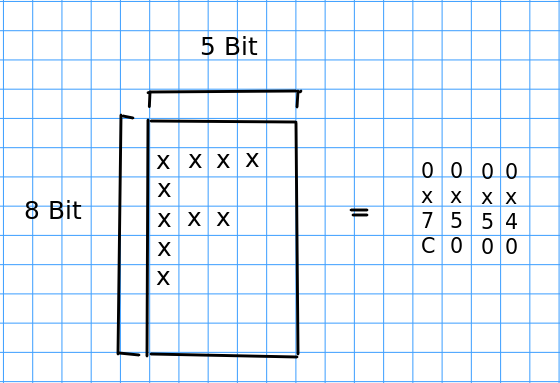
\includegraphics[width=0.7\textwidth]{media/char}
\end{center} \end{figure}

Mit diesem Format benötigt jedes Zeichen genau 5 Byte. Der Zeichensatz
enthält über 45 Zeichen, womit er insgesamt über 225 Byte an
Speicherplatz benötigt. Damit im Arbeitsspeicher kein wertvoller Platz  
verschwendet wird, ist der Zeichensatz mit der
{\tt pgmspace}-Erweiterung in den Programmspeicher ausgelagert.

Das Zeichenausgabe-Modul stellt die folgenden Prozeduren bereit:
\lstinputlisting{text.h}


\subsection{Helfer}


\subsubsection{Timer}

Das Timer-Modul stellt die folgenden Prozeduren bereit:
\lstinputlisting{timer.h}


\subsubsection{Assertions}

Das Assertion-Modul stellt die folgenden Prozeduren bereit:
\lstinputlisting{assert.h}


\subsection{Server}

Das Server-Modul ist in die folgenden, privaten Prozeduren unterteilt:
\lstinputlisting{main.c}


\section{Mobiltelefon}

\section{Projektumgebung}

\section{Lessons learned}

\section{Fazit}

\newpage

\appendix

\newpage

% include sources that are not cited explicitly
% \nocite{}

\bibliographystyle{plain}
\bibliography{article} 

\end{document}
